% Package
\documentclass[11pt]{article}

\usepackage{amsmath}
\usepackage{cite}
\usepackage{graphicx}
\usepackage[utf8]{inputenc}
\usepackage[T1]{fontenc}
\usepackage{lmodern}

\title{ADP Aufgabe 1, Abgabe 3}
\author{Team 1\\Hugo Protsch, Justin Hoffmann}

% Document
\begin{document}

    \maketitle


    \section{Formales}\label{sec:Formales}

    %! suppress = MissingLabel

    \subsection{Aufgabenaufteilung}
    Der Code wurde zusammen entwickelt.
    %! suppress = MissingLabel

    \subsection{Quellenangaben}

    Es wurden lediglich Vorlesungsmaterialien verwendet.

    %! suppress = MissingLabel

    \subsection{Bearbeitungszeitraum}
    Für die Bearbeitung und Überarbeitung des Entwurfs haben wir in etwa 10 bis
    12 Stunden benötigt.
    Für die Entwicklung des Quellcodes haben wir in etwa 15 bis 20 Stunden
    benötigt.
    %! suppress = MissingLabel

    \subsection{Aktueller Stand}
    Der Quellcode ist funktionsfähig und wurde auf Laufzeit überprüft.

    %! suppress = MissingLabel

    \subsection{Änderungen des Entwurfes}
    -- nicht zutreffend --


    \section{Laufzeitmessung}\label{sec:laufzeitmessung}

    \subsection{Zufällig}\label{subsec:zufaellig}

    \begin{center}
        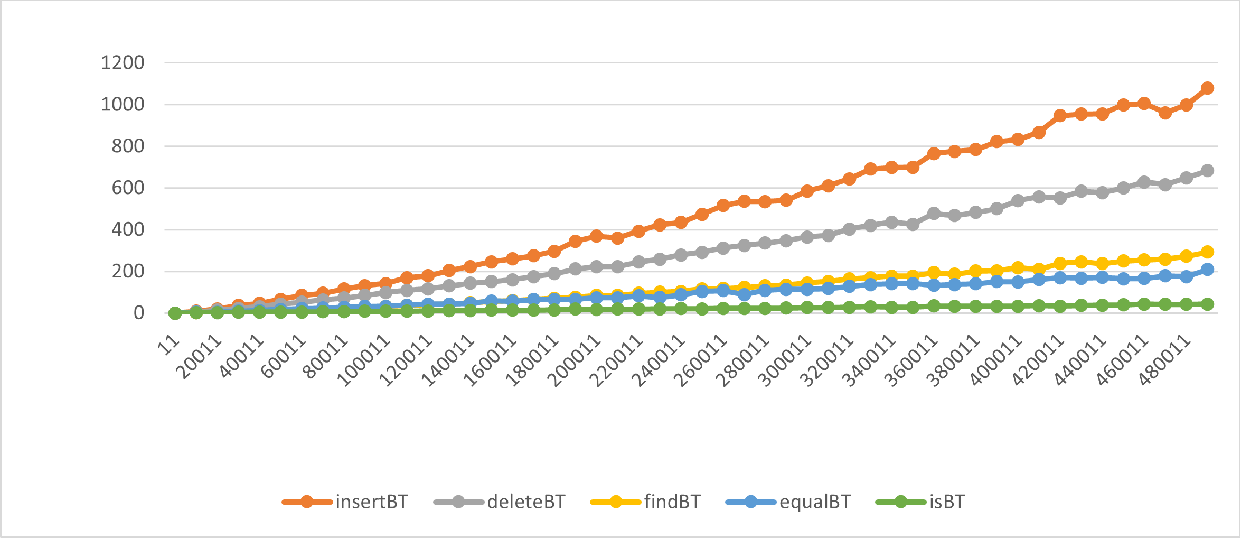
\includegraphics[width=0.9\columnwidth] {ZeitAvg.pdf}
    \end{center}

    Die Folgenden Einstellungen wurden bei der Messung verwendet:
    \begin{itemize}
        \item 0 Startelemente
        \item 1000 Elemente Schrittgröße
        \item 20 Schritte
        \item Mitteln über 5 Messungen
    \end{itemize}
    \begin{itemize}
        \item InsertBT:

        \item DeleteBT

        \item FindBT:

        \item EqualBT:

        \item IsBT:
    \end{itemize}

    \subsection{Aufsteigend und Absteigend}\label{subsec:average}

    \begin{center}
        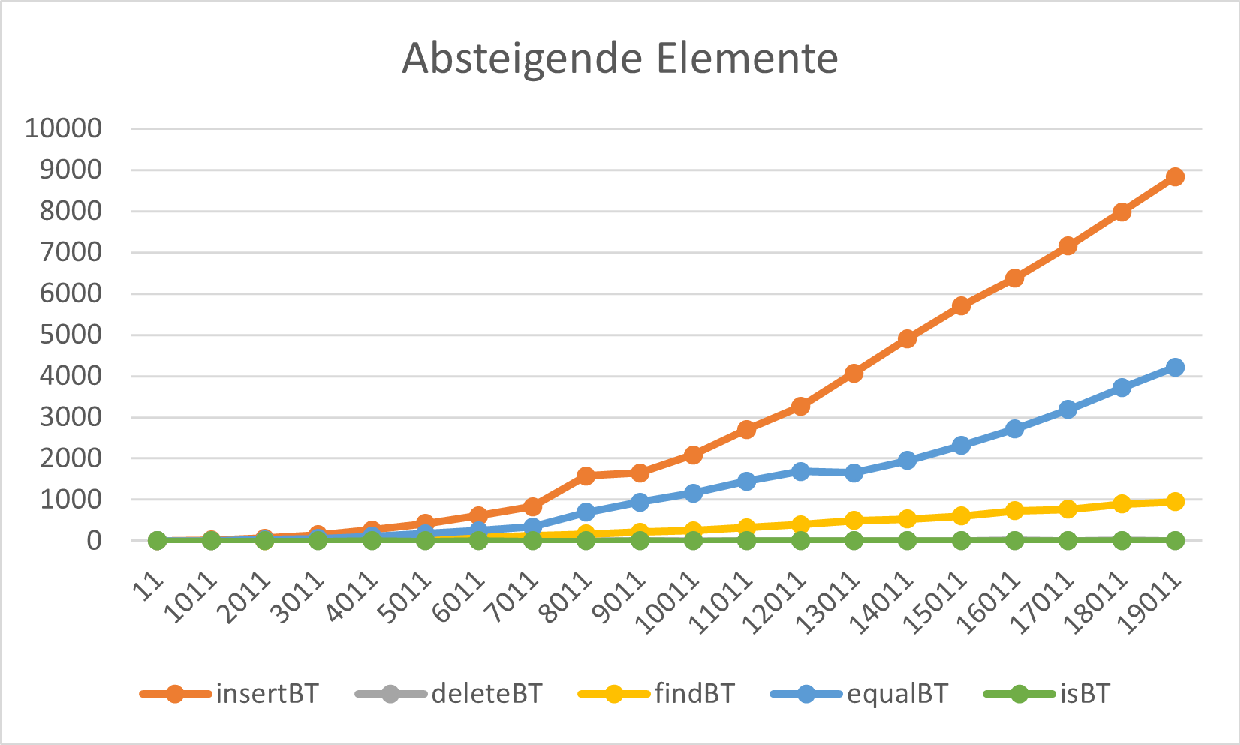
\includegraphics[width=0.9\columnwidth] {ZeitAb.pdf}
    \end{center}
    \begin{center}
        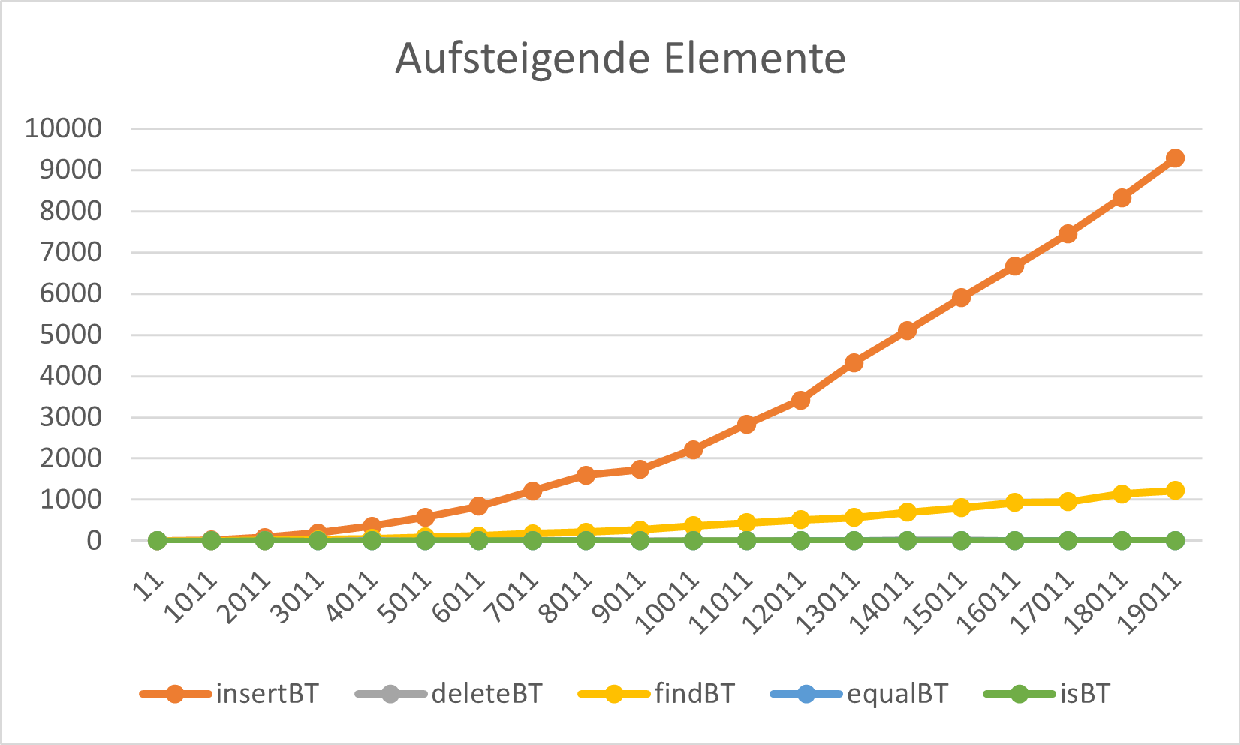
\includegraphics[width=0.9\columnwidth] {ZeitAuf.pdf}
    \end{center}

    Die Folgenden Einstellungen wurden bei der Messung verwendet:
    \begin{itemize}
        \item 0 Startelemente
        \item 10000 Elemente Schrittgröße
        \item 50 Schritte
        \item Mitteln über 10 Messungen
    \end{itemize}

    \begin{itemize}
        \item InsertBT:

        \item DeleteBT

        \item FindBT:

        \item EqualBT:

        \item IsBT:
    \end{itemize}


\end{document}
